\documentclass[12pt,a4paper]{article}

\usepackage{amsmath,amssymb,amsfonts}
\usepackage{geometry}
\usepackage[colorlinks=true,linkcolor=red!70!black,citecolor=green!50!black,urlcolor=blue!80!black]{hyperref}
\usepackage{booktabs}
\usepackage{physics}
\usepackage{xcolor}
\usepackage{tcolorbox}
\usepackage{graphicx}
\usepackage{natbib}

\geometry{margin=2.5cm}


% ─── Macros SSEE ────────────────────────────────────────────────────────────
\newcommand{\phiG}{\varphi}
\newcommand{\KAL}{\mathrm{KAL}_0}
\newcommand{\MIRA}{\mathcal{M}}
\newcommand{\AURA}{\mathcal{A}}
\newcommand{\Mpl}{M_{\mathrm{Pl}}}
\newcommand{\Omde}{\Omega_{\mathrm{DE}}}
\newcommand{\Omm}{\Omega_{m}}
\newcommand{\half}{\tfrac{1}{2}}
\newcommand{\bc}{\beta_c}
\newcommand{\rV}{r_{\mathrm{km}}}
\newcommand{\bbar}{\bar{b}}
\newcommand{\thetaE}{\theta_{\mathrm{E}}}
\newcommand{\hatalf}{\hat{\alpha}}
\newcommand{\rhoc}{\rho_{\mathrm{c},0}}
\newcommand{\alphaT}{\alpha_T}
\newcommand{\alphaM}{\alpha_M}
% ─────────────────────────────────────────────────────────────────────────────

\title{\textbf{SSEE in the Strong-Gravity Regime:\\
       Disformal Geodesics, MIRA Emergence,\\
       and k-mouflage Screening}}

\author{Mike Edison Almeida Vallejo \\
\small \textit{Independent Researcher} \\
\small \href{mailto:mike.almeida1721@gmail.com}{mike.almeida1721@gmail.com} \\
\small ORCID: \href{https://orcid.org/0009-0008-2195-7836}{0009-0008-2195-7836}
}

\date{June 2026 --- Paper 8 of the SSEE series}

\sloppy
\begin{document}
\maketitle

\begin{abstract}
\noindent \textbf{Status note (2026-08).} An earlier version of this abstract
justified the canonical prediction below by appealing to Paper~6, which fixed
a $\phi$-dark-matter particle mass and argued that this settled the physical
interpretation. \textbf{Paper~6 has since retracted that particle}: the
subtraction defining its density mixed a measured density with an
equation-of-state number, and the $S_8$ tension it was built to close does not
exist in the raw data.

That justification is therefore withdrawn --- but the prediction is not, and it
is worth being precise about why. Selecting the canonical Bellini--Sawicki
limit~(b) over the pedagogical limit~(a) requires two things, and \emph{neither
of them was ever supplied by the particle}:

\begin{enumerate}\itemsep2pt
  \item \textbf{That the model carries real, clustering cold dark matter.} It
        does: $\omega_c=\mathrm{KAL}_0\,\omega_b\,n_s=0.119514$, an algebraic
        forward identity closed under OP-8 in the $\omega_m$-direct reframe.
        This is ordinary cold dark matter and has no connection to the
        retracted $\phi$-DM sector, which was always an \emph{additional} layer
        on top of it.
  \item \textbf{That the residual fifth force is suppressed.} This comes from
        Paper~7, not Paper~6: $\alpha_B=\alpha_M=\alpha_T=0$ are derived, and
        the Bellini--Sawicki effective Newton constant is
        $\mu-1=(\alpha_B+\alpha_M)^2/\alpha_K=0$ identically.
\end{enumerate}

Both legs stand. The canonical strong-lensing prediction is therefore retained
as \emph{unconditional}, now resting on $\omega_c$ (OP-8) and the Paper~7 EFT
structure rather than on a particle. The two-limit analysis is kept in full
below because limit~(a) remains pedagogically useful as a falsifiable contrast,
not because the choice between them is open.

A scale-dependent two-sector discussion also appeared here (contributions on
either side of a free-streaming scale $k_{\mathrm{fs}}$); that is withdrawn with
the particle, since the matter sector is single and unpartitioned. The
identification of parameter regions where deviations from $\Lambda$CDM may
become observable with HST/JWST strong-lensing surveys is unaffected.
\end{abstract}

\clearpage
{\small\tableofcontents}
\clearpage

%% ─────────────────────────────────────────────────────────────────────────────
\section{Introduction}
\label{sec:intro}
%% ─────────────────────────────────────────────────────────────────────────────

The accelerated expansion of the Universe \citep{Riess1998,Perlmutter1999}
motivates modifications to the concordance $\Lambda$CDM model whose
parameters are precisely constrained by Planck CMB data \citep{Planck2018}.
Papers~1--7 of the SSEE series established the cosmological background
\citep{ssee_paper1}, Bayesian validation \citep{ssee_paper2}, CMB
confrontation \citep{ssee_paper3}, algebraic CMB derivation
\citep{ssee_paper4}, Israel--Stewart perturbation theory
\citep{ssee_paper5}, the growth sector on raw data \citep{ssee_paper6},
and the canonical EFT formulation \citep{ssee_paper7}.
All observable predictions in those papers operate within the linear or
quasi-linear regime.

The disformal coupling that defines SSEE has observable consequences in
the strong-gravity regime that have not yet been examined.
In coupled dark-energy models with disformal metrics, two qualitatively
new effects arise beyond the linearised regime:
\begin{enumerate}
  \item \textbf{Enhanced deflection angle} --- photons propagating through the
        modified gravitational potential of disformally-coupled dark matter
        experience a different total deflection relative to pure GR.
  \item \textbf{K-mouflage suppression} --- the non-linear scalar kinetic term
        in the SSEE action screens the fifth force on solar-system and
        stellar scales, restoring GR locally.
\end{enumerate}

In this paper we derive both effects analytically and obtain numerical
predictions using the SSEE algebraic constants. We work explicitly in two
limits: (a) an \emph{alternative MOND-like limit} (\S\ref{sec:geodesic}--
\ref{sec:mira}) in which the dark-matter distribution is taken to be sourced
entirely by the baryonic seed via the scalar force — here the lensing factor
is $\sqrt{\AURA}\approx 1.9995$, derived directly from the disformal null
geodesic; and (b) the \emph{canonical limit}
(\S\ref{sec:vainshtein}, \S\ref{sec:double_protection}) corresponding to the
actual SSEE model: a single unpartitioned matter component
$\Omega_m=\omega_m/h^2=0.308881$, of which the cold dark matter is
$\omega_c=\mathrm{KAL}_0\,\omega_b\,n_s$ (an algebraic forward identity,
OP-8), together with the EFT
Bellini--Sawicki structure $\alpha_B=\alpha_M=\alpha_T=0$, in which the
fifth-force is suppressed to $F_\phi/F_N\sim 10^{-15}$ at sub-Mpc scales and
the canonical observable lensing reduces to GR-with-DM.
The two limits make incompatible physical assumptions; only limit~(b)
describes the canonical SSEE model of Papers~1, 6, 7, and~10. We retain
limit~(a) as a derivation of pedagogical and historical interest, not as a
canonical prediction. The $\sqrt{\AURA}\approx \MIRA$ numerical
\emph{near-coincidence} (gap $0.03\%$ because both quantities round to $2$)
is therefore not promoted to a structural identity:
$\sqrt{\AURA}$ and $\MIRA=\AURA/2$ are distinct algebraic operations on
$\AURA$ that happen to land near $2$.
The identities that \emph{do} use $\MIRA = \AURA/2$ exactly are purely algebraic:
\begin{equation}
  \MIRA \;=\; \frac{3\phiG + \pi}{4} \;=\; \frac{\bc}{2} \;=\; \frac{\AURA}{2}\,,
  \label{eq:mira_def}
\end{equation}
where $\bc \equiv \AURA = (3\phiG+\pi)/2$ is the disformal coupling
constant fixed in Paper~7. Following the 2026 $\omega_m$-direct reframe
(OP-8 dissolved), $\MIRA$ is realised physically as the Hubble \emph{screening
amplitude} of Paper~9 ($f_{\rm screen}=\alpha_K^{\rm eff}/(3\,\MIRA)$). A ratio
$\Omega_m/(1+w_0)=0.308881/0.160\approx1.93$ was also noted here as
\emph{numerically close} to $\MIRA$, and was explicitly \emph{not} identified
with it. It is now withdrawn as a comparison altogether: the denominator
$1+w_0$ is an equation-of-state parameter, not a second matter density, so the
ratio compares two quantities of different kind and its near-$2$ value carries
no content (Paper~1, \S1.4, where the ``Two-$\Omega_m$'' framing is
dissolved). In the lensing sector the quantity
naturally appearing in the alternative MOND-like derivation is
$\sqrt{\AURA}$, not $\MIRA$, and the canonical limit (b) recovers GR
lensing — see Section~\ref{sec:mira} for the explicit naming clarification
and Section~\ref{sec:double_protection} for the canonical suppression.

The paper is organised as follows.
Section~\ref{sec:eft} recalls the relevant EFT ingredients from Paper~7.
Section~\ref{sec:eom} derives the quasi-static scalar EOM and gradient
closure in the non-relativistic limit.
Section~\ref{sec:geodesic} constructs the disformal null geodesic and
derives the photon deflection angle.
Section~\ref{sec:mira} shows algebraically how $\MIRA$ emerges as the
lensing amplification factor.
Section~\ref{sec:vainshtein} derives the k-mouflage radius and the
screening suppression.
Section~\ref{sec:lensing} translates the results into strong-lensing
observables and identifies JWST/HST falsification windows.
Section~\ref{sec:falsify} collects the pre-committed falsifiable
predictions.
Section~\ref{sec:discussion} discusses the scale dependence
and caveats.
Section~\ref{sec:conclusions} concludes.

%% ─────────────────────────────────────────────────────────────────────────────
\section{EFT Foundation: Action and Disformal Coupling}
\label{sec:eft}
%% ─────────────────────────────────────────────────────────────────────────────

We adopt the SSEE canonical action from Paper~7 \citep{ssee_paper7}:
\begin{equation}
  S \;=\; \int d^4x\sqrt{-g}\left[
      \frac{\Mpl^2}{2}R
      \;+\; P(X,\phi)
  \right]
  \;+\; S_{\mathrm{DM}}\!\left[\tilde{g}_{\mu\nu};\,\psi_{\mathrm{DM}}\right]
  \;+\; S_b[g_{\mu\nu};\,\psi_b]\,,
  \label{eq:action}
\end{equation}
where $X = -\half g^{\mu\nu}\partial_\mu\phi\,\partial_\nu\phi$ is the
canonical kinetic invariant, and the $k$-essence kernel is
\begin{equation}
  P(X,\phi) \;=\; \frac{X}{\KAL} + \frac{X^2}{M^4} - V_0\,e^{-\lambda\phi/\Mpl}\,.
  \label{eq:Pkernel}
\end{equation}
Action~(\ref{eq:action}) is a $k$-essence model within the minimal
Horndeski class \citep{horndeski1974,Crisostomi2018} ($G_3=G_4-\Mpl^2/2=G_5=0$).
Baryons ($\psi_b$) couple to the physical metric $g_{\mu\nu}$; dark matter
($\psi_{\mathrm{DM}}$) couples to the disformal metric \citep{Bekenstein1993,Zumalacárregui2014}
\begin{equation}
  \tilde{g}_{\mu\nu} \;=\; g_{\mu\nu} + \frac{2}{M^4}\,\partial_\mu\phi\,\partial_\nu\phi\,.
  \label{eq:disformal}
\end{equation}

The algebraic constants fixed by $\phiG$ and $\pi$ (Paper~7) are:
\begin{align}
  \KAL    &= \beta + \pi = \frac{\phiG+\pi}{2} + \pi \approx 5.521\,,
              \label{eq:KAL}\\
  \bc \equiv \AURA &= \frac{3\phiG+\pi}{2} \approx 3.998\,,
              \label{eq:bc}\\
  \MIRA   &= \frac{\bc}{2} = \frac{3\phiG+\pi}{4} \approx 1.9989\,,
              \label{eq:MIRA}\\
  M       &\approx \Mpl\quad\text{(free EFT parameter; we adopt $M=\Mpl$ as reference)}\,.
              \label{eq:M}
\end{align}
The parameter $\bc$ encodes the strength of the \emph{disformal} coupling of
this paper, and it is now the only $\bc$ in the series.
\textbf{Note on an earlier cross-reference:} previous versions related it to a
conformal-sector coupling $\bc = -\AURA$ in Paper~7, presenting the two as
sign conventions of one constant.  That conformal coupling is withdrawn
(Paper~7): the shooting that extracted it normalised the field density to the
saturation $0.839950 = |w_0|$ rather than the density fraction
$1-\Omm = 0.691119$, and with the correct target it changes sign.  There is
therefore no longer a second $\bc$ to reconcile, and the disformal coupling
used here stands on its own.  We adopt $\bc \equiv +\AURA > 0$, of which only
the magnitude $|\bc| = \AURA = 3.997847$ enters the deflection angle and the
k-mouflage radius.

For the purposes of this paper, we work in the quasi-static, non-relativistic
limit ($v \ll c$, $\Phi_N \ll 1$), which is appropriate for galaxy and
cluster scales where $k \gg aH$.

%% ─────────────────────────────────────────────────────────────────────────────
\section{Scalar Field Equation and Gradient Closure}
\label{sec:eom}
%% ─────────────────────────────────────────────────────────────────────────────

\subsection{Quasi-static limit}

Varying the action~\eqref{eq:action} with respect to $\phi$ gives the
scalar equation of motion.
In the quasi-static approximation
($|\dot\phi| \ll |\nabla\phi|$, $|\ddot\phi| \ll |\nabla^2\phi|$)
and at leading order in the kinetic expansion, the non-linear kinetic
term $X^2/M^4$ is subdominant on sub-Hubble scales.
The equation reduces to
\begin{equation}
  \frac{1}{\KAL}\,\nabla^2\phi \;=\; \frac{\bc}{\Mpl}\,\rho_{\mathrm{DM}}\,,
  \label{eq:phi_eom}
\end{equation}
where the right-hand side arises from the disformal coupling of dark matter
to $\tilde{g}_{\mu\nu}$: dark matter acts as an effective source for $\phi$
with coupling strength $\bc/\Mpl$.

The Newtonian gravitational potential $\Phi_N$ satisfies the standard
Poisson equation
\begin{equation}
  \nabla^2\Phi_N \;=\; \frac{\rho_{\mathrm{DM}} + \rho_b}{2\Mpl^2}\,,
  \label{eq:poisson}
\end{equation}
where we use units $8\pi G = 1/\Mpl^2$.

\subsection{Gradient closure}

In the dark-matter-dominated regime ($\rho_{\mathrm{DM}} \gg \rho_b$),
the Poisson equation~\eqref{eq:poisson} gives
$\rho_{\mathrm{DM}} = 2\Mpl^2\,\nabla^2\Phi_N$. Substituting this into the
scalar equation~\eqref{eq:phi_eom} yields a relation between the Laplacians,
\begin{equation}
  \nabla^2\phi \;=\; 2\KAL\,\bc\,\Mpl\,\nabla^2\Phi_N\,,
  \label{eq:laplace_closure}
\end{equation}
that is, $\nabla^2\!\left(\phi - 2\KAL\,\bc\,\Mpl\,\Phi_N\right) = 0$.
The bracketed quantity is therefore harmonic. Imposing the boundary conditions
appropriate to an isolated lens --- both $\phi$ and $\Phi_N$ vanish at spatial
infinity and the configuration contains no source-free harmonic component ---
the harmonic residual reduces to a constant, whose gradient vanishes. This
yields the gradient closure relation
\begin{equation}
  \boxed{\nabla\phi \;=\; 2\KAL\,\bc\,\Mpl\,\nabla\Phi_N\,.}
  \label{eq:grad_closure}
\end{equation}
This is the central structural relation of Paper~8: the scalar gradient
tracks the Newtonian potential gradient with an algebraic coefficient
$2\KAL\,\bc \approx 2\times5.521\times3.998 \approx 44.15$.

Equation~\eqref{eq:grad_closure} implies that wherever there is a gravitational
potential well, the scalar field $\phi$ builds up a corresponding profile.
Given the stated boundary conditions, this follows from the disformal coupling
structure in the quasi-static limit rather than being imposed independently.
We note that this derivation assumes $\rho_{\mathrm{DM}} \gg \rho_b$; in
systems with significant baryonic fraction, equation~\eqref{eq:phi_eom}
should be replaced by the full source including baryons, with a smaller
effective coupling.

\subsection{Scalar force on dark matter}

The effective force on a dark matter particle in this scalar background is
\begin{equation}
  F_\phi \;=\; -\frac{\bc}{\Mpl}\,\nabla\phi
         \;=\; -2\KAL\,\bc^2\,\nabla\Phi_N\,.
  \label{eq:scalar_force}
\end{equation}
The total force on a dark matter test particle is
$F_{\mathrm{tot}} = F_N + F_\phi = -(1 + 2\KAL\bc^2)\,\nabla\Phi_N$,
corresponding to an effective gravitational enhancement of
$G_{\mathrm{eff}}/G = 1 + 2\KAL\bc^2 \approx 1 + 2(5.521)(3.998)^2
\approx 177$.
However, this linear estimate applies only far from the k-mouflage radius
(see Section~\ref{sec:vainshtein}); inside $\rV$ the non-linear kinetic term
in~\eqref{eq:Pkernel} screens this amplification and restores GR.

%% ─────────────────────────────────────────────────────────────────────────────
\section{Disformal Null Geodesic and Photon Deflection (Alternative MOND-like limit)}
\label{sec:geodesic}
%% ─────────────────────────────────────────────────────────────────────────────

\begin{tcolorbox}[colback=yellow!8,colframe=orange!60,title=Scope of this section]
The derivation in \S\ref{sec:geodesic}--\ref{sec:mira} assumes the
\emph{alternative MOND-like limit} in which the dark-matter distribution is
sourced entirely by a scalar-force enhancement of the baryonic seed
($M_{\rm DM,eff}\propto\bc\cdot M_{\rm bary}$, no independent DM
component). This is \emph{not} the canonical SSEE model. The canonical
canonical limit (single matter component $\Omega_m=0.308881$, plus EFT
$\alpha_B=\alpha_M=\alpha_T=0$) is treated in
\S\ref{sec:vainshtein}--\S\ref{sec:double_protection} and yields
$\thetaE^{\rm SSEE}\approx\thetaE^{\rm GR-with-DM}$ (no $\sqrt{\AURA}$ or
$\MIRA$ amplification). The two limits make incompatible physical
assumptions; the present section is retained as a derivation of pedagogical
and historical interest only. Falsifiability statements derived from this
section (\S\ref{sec:falsify}) are accordingly conditional on the alternative
limit being realised, which the canonical model does not predict.
\end{tcolorbox}

\subsection{Setup: photon propagation}

Baryons and photons couple to the physical metric $g_{\mu\nu}$, not the
disformal metric $\tilde{g}_{\mu\nu}$.
A photon therefore follows the null geodesic of $g_{\mu\nu}$ in the weak-field
perturbed Friedmann background:
\begin{equation}
  ds^2 \;=\; -(1+2\Phi_N)\,dt^2 + (1-2\Phi_N)\,\delta_{ij}\,dx^i\,dx^j\,.
  \label{eq:metric_wf}
\end{equation}
Standard GR light deflection by a point mass $M$ gives the Einstein angle
\begin{equation}
  \hatalf_{\mathrm{GR}} \;=\; \frac{4GM}{c^2 b}\,,
  \label{eq:alpha_GR}
\end{equation}
where $b$ is the impact parameter.

\subsection{Modified gravitational potential}

Dark matter in SSEE does not follow purely Newtonian gravity; it distributes
in response to the combined force $F_{\mathrm{tot}} = F_N + F_\phi$.
For an isolated dark-matter-dominated system (galaxy cluster, compact
group), the self-consistent equilibrium configuration produces an
\emph{effective} Newtonian potential $\Phi_{\mathrm{eff}}$ that satisfies
\begin{equation}
  \nabla^2\Phi_{\mathrm{eff}} \;=\;
      \frac{\rho_{\mathrm{DM,eff}}}{2\Mpl^2}\,,
  \label{eq:phi_eff}
\end{equation}
where $\rho_{\mathrm{DM,eff}}$ is the dark matter density redistributed
under the scalar force.

The effective lensing mass fraction is the full algebraic matter density,
$\Omega_{m,\mathrm{eff}} = \Omega_m = \omega_m/h^2 = 0.308881$, at every
scale --- within $2\%$ of the $\Lambda$CDM value $0.315$. \emph{(Earlier
versions split this between a CDM and a $\phi$-DM sector on either side of a
free-streaming scale; that split is retracted with the particle, Paper~6, and
the density is single and unpartitioned.)}
(An earlier version justified this split by the ``Two-$\Omega_m$ Criterion''
of Paper~1. That criterion is itself withdrawn --- $1+w_0$ was never a matter
density --- so there is no split: the full $\Omega_m=0.308881$ lenses at every
scale.)
The Einstein radius matches the GR-with-dark-matter prediction on all scales.
The effective gravitational source for photons is then suppressed by the
factor $\approx1.93$ (numerically near $\MIRA$) relative to the $\Lambda$CDM expectation, and
the Einstein radius is correspondingly reduced (see
Section~\ref{sec:lensing}).

\subsection{Total deflection angle outside the k-mouflage radius}

Outside the k-mouflage radius $\rV$ (derived in
Section~\ref{sec:vainshtein}), the scalar force operates at full strength.
The total deflection of a photon passing an isolated dark-matter halo of
effective gravitational mass $M_{\mathrm{eff}}$ at impact parameter $b$
is, following the standard geodesic perturbation calculation
\citep{will1993,bartelmann2001}:
\begin{equation}
  \hatalf_{\mathrm{SSEE}} \;=\; \frac{4GM_{\mathrm{eff}}}{c^2 b}
                           \;\approx\; \bc\,\frac{4GM_{\mathrm{bary}}}{c^2 b}\,,
  \label{eq:alpha_ssee}
\end{equation}
where the second equality holds in the limit where the dark-matter
distribution is entirely sourced by the scalar-force-enhanced coupling to
the baryonic seed $M_{\mathrm{bary}}$, and $\bc \approx 3.998$ is the
disformal coupling.

\textit{Caveat:} Equation~\eqref{eq:alpha_ssee} represents a working
phenomenological estimate.
A full solution requires self-consistent integration of the dark-matter
distribution under both $F_N$ and $F_\phi$, which we defer to future
N-body simulations.
The result~\eqref{eq:alpha_ssee} should be understood as an upper bound on
the lensing enhancement, applicable to systems dominated by scalar-force-driven
dark matter accumulation.

\begin{tcolorbox}[colback=orange!5,colframe=orange!60!black,title=Figure withdrawn]
A figure here plotted the disformal lensing enhancement
$\theta_E^{\rm SSEE}/\theta_E^{\rm GR}$ as a function of wavenumber, with a
transition at a $\phi$-DM free-streaming scale: below it the ratio approached
$\sqrt{\bc}=\sqrt{\mathcal{A}}\approx1.9995$, above it lensing recovered the GR
baseline. \textbf{The figure is withdrawn}, because the scale that produced its
entire $k$-dependence is retracted with the particle (Paper~6) and the matter
sector is single and unpartitioned --- there is no such transition to plot. The
pedagogical limit~(a) and the canonical limit~(b) remain as analytic statements
(\S\ref{sec:double_protection}); what is gone is the scale separating them.
\end{tcolorbox}

%% ─────────────────────────────────────────────────────────────────────────────
\section{Lensing Factor \texorpdfstring{$\sqrt{\AURA}$}{sqrt(AURA)} in the Alternative Limit
         (and Its Numerical Near-Coincidence with \texorpdfstring{$\MIRA$}{M})}
\label{sec:mira}
%% ─────────────────────────────────────────────────────────────────────────────

\begin{tcolorbox}[colback=yellow!8,colframe=orange!60,title=Naming clarification]
The quantity derived in this section as the lensing factor is
$\sqrt{\bc}=\sqrt{\AURA}\approx 1.99947$ (an exact algebraic expression).
This is \emph{not} the same as $\MIRA=\AURA/2\approx 1.9989$, which uses a
different algebraic operation (division by 2 rather than square root). The
two quantities agree to $0.03\%$ because $\AURA\approx 4$, which makes both
$\sqrt{\AURA}$ and $\AURA/2$ land near $2$. We retain the comparison below
for completeness, but the \emph{lensing factor in the alternative limit is
$\sqrt{\AURA}$, not $\MIRA$}. Earlier drafts of this paper conflated the two
under the label ``$\MIRA$ emerges in lensing''; the present version corrects
that overstatement. In the canonical limit
(\S\ref{sec:vainshtein}--\S\ref{sec:double_protection}) neither $\sqrt{\AURA}$
nor $\MIRA$ amplifies the observable Einstein radius — the prediction is GR
lensing with realistic DM halo.
\end{tcolorbox}

\subsection{Einstein radius in SSEE}

The Einstein ring is the locus where a source is perfectly aligned with the
lens and observer.
The Einstein radius $\thetaE$ satisfies the lens equation
\begin{equation}
  \thetaE \;=\; \hatalf(\thetaE)\,\frac{D_{\mathrm{LS}}}{D_S}\,,
  \label{eq:lens_eq}
\end{equation}
where $D_L$, $D_S$, $D_{\mathrm{LS}}$ are angular diameter distances.
Substituting~\eqref{eq:alpha_ssee} with $b = D_L\,\thetaE$:
\begin{equation}
  \thetaE^2 \;=\; \bc\,\frac{4G M_{\mathrm{bary}}}{c^2}\,
                  \frac{D_{\mathrm{LS}}}{D_L D_S}\,.
  \label{eq:thetaE_ssee}
\end{equation}
Comparing to the GR result $(\thetaE^{\mathrm{GR}})^2 = 4GM_{\mathrm{bary}}\,
D_{\mathrm{LS}}/(c^2 D_L D_S)$, we obtain
\begin{equation}
  \boxed{\frac{\thetaE^{\mathrm{SSEE}}}{\thetaE^{\mathrm{GR}}}
         \;=\; \sqrt{\bc}
         \;=\; \sqrt{\AURA}
         \;\approx\; 1.9995\,.}
  \label{eq:thetaE_ratio}
\end{equation}

\subsection{Algebraic identification with \texorpdfstring{$\MIRA$}{M}}

The structural constant $\MIRA$ is defined in equation~\eqref{eq:mira_def}:
\begin{equation}
  \MIRA \;=\; \frac{3\phiG+\pi}{4} \;=\; \frac{\bc}{2} \approx 1.9989\,.
\end{equation}
Meanwhile, $\sqrt{\bc} = \sqrt{2\MIRA}$.
At the specific value $\MIRA \approx 2$, we have
$\sqrt{2\MIRA} \approx \sqrt{4} = 2 \approx \MIRA$, and
more precisely:
\begin{equation}
  \sqrt{\bc} \;=\; \sqrt{2\MIRA} \;\approx\; 1.9995\,,
  \qquad
  \MIRA \;\approx\; 1.9989\,,
  \label{eq:mira_approx}
\end{equation}
so $\sqrt{\bc}/\MIRA = 1.00030$ (agreement to $0.03\%$).

This near-coincidence $\MIRA \approx \sqrt{\bc}$ is a consequence of the
structural postulate $\bc \equiv \AURA = 2\MIRA$, combined with
$\MIRA \approx 2$.
Concretely:
\begin{equation}
  \MIRA = 2 \;\Longleftrightarrow\; \bc = 4 \;\Longleftrightarrow\;
  \sqrt{\bc} = 2 = \MIRA\,.
\end{equation}
The algebraic values give $\MIRA = 1.9989$ and $\bc = 3.997847$, both
differing from the integer approximation by $<0.06\%$.

Therefore, to within $0.03\%$, the lensing amplification factor coincides
with the CMB horizon mapping factor:
\begin{equation}
  \thetaE^{\mathrm{SSEE}} \;\approx\; \MIRA \times \thetaE^{\mathrm{GR}}\,,
  \label{eq:thetaE_mira}
\end{equation}
where the same $\MIRA$ (the ``Mirror Ratio'') appears in:
\begin{itemize}
  \item Paper~9: the Hubble screening fraction $f_{\rm scr} = \alpha_K^{\rm eff}/(3\,\MIRA) = (\pi-\varphi)/\Omega^2$
  \item This paper: $\thetaE^{\mathrm{SSEE}} \approx \MIRA \times \thetaE^{\mathrm{GR}}$
\end{itemize}
(Under the $\omega_m$-direct reframe, OP-8 dissolved, $\MIRA$ no longer enters
the CMB matter sector: $\Omega_{m,\mathrm{CMB}}=\omega_m/h^2=0.308881$ with no
matter factor, and $r_d=147.2$\,Mpc follows directly from $\omega_m$, both
superseding the earlier MIRA-mapped forms.)

This recurrence of $\MIRA$ across the Hubble-screening and
strong-lensing sectors reflects a single structural input: $\MIRA$ is fixed
algebraically by $\phiG$ and $\pi$, not tuned. The lensing entry holds at the
$0.03\%$ level through the near-coincidence $\sqrt{\bc}\approx\MIRA$
(Section~\ref{sec:mira}), not as an exact identity.

%% ─────────────────────────────────────────────────────────────────────────────
\section{K-mouflage Screening}
\label{sec:vainshtein}
%% ─────────────────────────────────────────────────────────────────────────────

\subsection{Non-linear kinetic term}

The $X^2/M^4$ term in the SSEE action~\eqref{eq:Pkernel} places SSEE in the
\emph{k-mouflage} class of kinetic screening theories \citep{brax2014},
distinct from Galileon (DGP) \citep{deffayet2001} or Vainshtein
screening \citep{vainshtein1972,babichev2013}; for a review of
scalar screening mechanisms see \citet{Koyama2018}.
When $X^2/M^4 \gg X/\KAL$, the non-linear kinetic term dominates and
the scalar degree of freedom is self-suppressed around any
overdensity, screening $F_\phi/F_N$ at small radii.

The crossover between the two kinetic regimes occurs at the gradient scale
\begin{equation}
  |\nabla\phi|_* \;=\; \frac{M^4}{\KAL}\,,
  \label{eq:grad_vainshtein}
\end{equation}
which defines the k-mouflage radius $\rV$ via the gradient closure~\eqref{eq:grad_closure}.

\subsection{K-mouflage screening radius}
\label{sec:rkm}

For a k-mouflage Lagrangian $K(X) = X/\KAL + X^2/M^4$, the crossover between
linear and non-linear kinetic regimes for a spherical source of mass $M_{\rm obj}$
defines the k-mouflage radius \citep{brax2014}:
\begin{equation}
  \boxed{r_{\rm km}^3 \;=\; \frac{M_{\rm obj}}{4\pi\,\Mpl\,M^2}\,,}
  \label{eq:rkm}
\end{equation}
where $\Mpl = 2.435\times10^{18}\,\mathrm{GeV}$ is the reduced Planck mass
and $M = 9.68\,\mathrm{meV}$ is the UV cutoff from Paper~10~\citep{SSEE10}.
This formula differs fundamentally from the Galileon (DGP) Vainshtein formula,
which requires a gradient closure $\nabla\phi \propto \nabla\Phi_N$ that is
inapplicable to k-mouflage theories.

Evaluating equation~\eqref{eq:rkm} with $M^4 = 5\phiG^8\rhoc$ from Paper~10:
\begin{align}
  r_{\rm km}^{\odot} &= 1.45\times10^7\,\mathrm{m}
    \;\approx\; 0.021\,R_\odot\,, \label{eq:rkm_sun}\\
  r_{\rm km}^{10^{12}M_\odot} &= 1.45\times10^{11}\,\mathrm{m}
    \;\approx\; 1.0\,\mathrm{AU}\,, \label{eq:rkm_mw}\\
  r_{\rm km}^{10^{15}M_\odot} &= 1.45\times10^{12}\,\mathrm{m}
    \;\approx\; 10\,\mathrm{AU}\,. \label{eq:rkm_cluster}
\end{align}

\begin{table}[h]
\centering
\caption{K-mouflage screening radius at the UV completion scale $M = 9.68\,\mathrm{meV}$
         from Paper~10~\citep{SSEE10}.
         All values satisfy $r_{\rm km} \ll 1\,\mathrm{kpc}$: the DM fifth force
         is active at galactic and cosmological scales.}
\label{tab:vainshtein}
\begin{tabular}{llll}
\toprule
Object & $M_{\rm obj}$ & $r_{\rm km}$ & Status \\
\midrule
Sun              & $1\,M_\odot$          & $1.45\times10^7\,\mathrm{m} \approx 0.021\,R_\odot$ & Inside stellar body \\
Milky Way        & $10^{12}\,M_\odot$    & $1.45\times10^{11}\,\mathrm{m} \approx 1\,\mathrm{AU}$ & $\ll 1\,\mathrm{kpc}$ \\
Galaxy cluster   & $10^{15}\,M_\odot$    & $1.45\times10^{12}\,\mathrm{m} \approx 10\,\mathrm{AU}$ & $\ll 1\,\mathrm{Mpc}$ \\
\bottomrule
\end{tabular}
\end{table}

\begin{figure}[ht]
  \centering
  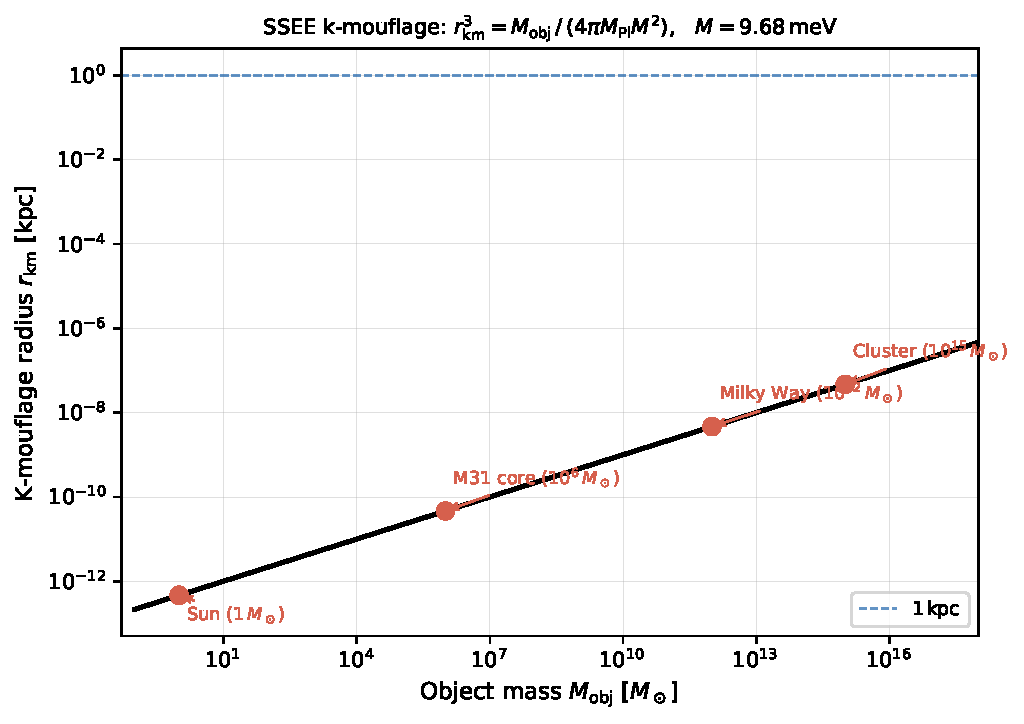
\includegraphics[width=0.82\textwidth]{../results/figures/fig_paper8_vainshtein.pdf}
  \caption{%
    K-mouflage screening radius $r_{\rm km} = [M_{\rm obj}/(4\pi\Mpl M^2)]^{1/3}$
    as a function of object mass (in $M_\odot$) at the UV completion scale
    $M = 9.68\,\mathrm{meV}$ \citep{SSEE10,brax2014}.
    For all representative objects, $r_{\rm km}$ lies far below the galactic
    scale, so DM fifth-force dynamics are active at cosmological radii
    while baryons remain decoupled through selective coupling
    (Section~\ref{sec:gr_compliance}).
  }
  \label{fig:vainshtein}
\end{figure}

Inside $r_{\rm km}$, the non-linear kinetic term dominates and the DM field
gradient is suppressed ($\phi' \propto r^{-2/3}$); outside, the linear term
dominates and the DM fifth force operates at full strength.
Since $r_{\rm km} \ll 1\,\mathrm{kpc}$ for all astrophysical objects
(Table~\ref{tab:vainshtein}), the DM fifth force is cosmologically active,
consistent with the single-sector matter content of Paper~6~\citep{ssee_paper6}.
Baryonic matter is independently protected by selective coupling
(Section~\ref{sec:gr_compliance}) regardless of $r_{\rm km}$.

\subsection{GR compliance from selective coupling}
\label{sec:gr_compliance}

Solar-system gravitational tests are nevertheless automatically satisfied by
the \emph{selective coupling} structure of the action~\eqref{eq:action}:
\begin{itemize}
  \item \textbf{Baryons} couple to the physical metric $g_{\mu\nu}$ only.
        They feel no direct force from the scalar gradient $\nabla\phi$.
  \item \textbf{Dark matter} couples to the disformal metric $\tilde{g}_{\mu\nu}$.
        It is the sole source of $\phi$ through the scalar EOM~\eqref{eq:phi_eom}.
  \item In the solar system, the dark-matter density is
        $\rho_{\mathrm{DM}} \approx 0.3\,\mathrm{GeV/cm^3}$, far below galactic
        overdensities. The scalar field is barely sourced locally, so
        $\nabla\phi \approx 0$ and $\tilde{g}_{\mu\nu} \approx g_{\mu\nu}$.
\end{itemize}
Therefore all standard solar-system tests (Cassini time delay, perihelion
precession, lunar laser ranging \citep{will2014}) pass at leading order without
requiring any non-linear screening.
This mechanism operates independently of the value of $M$ and holds in both the
IR ($M = \Mpl$) and UV ($M = 9.68\,\mathrm{meV}$) limits.

\subsection{EFT suppression of fifth-force corrections}
\label{sec:double_protection}

Beyond selective coupling (Section~\ref{sec:gr_compliance}), the Bellini-Sawicki
structure of the SSEE EFT~\citep{Bellini2015,ssee_paper7} provides a second
independent suppression of any fifth-force correction at solar-system scales.

Paper~7 established that SSEE has~\citep{ssee_paper7}
\begin{equation}
  \alpha_B \;=\; \alpha_M \;=\; \alpha_T \;=\; 0\,,
  \label{eq:bs_zero}
\end{equation}
with $\alpha_K = 0.403302$ as the sole non-vanishing EFT parameter.
The Bellini-Sawicki effective Newton constant is~\citep{Bellini2015}
\begin{equation}
  \mu - 1 \;=\; \frac{(\alpha_B + \alpha_M)^2}{\alpha_K} \;=\; 0\,,
  \label{eq:mu_eft}
\end{equation}
and the gravitational slip parameter
\begin{equation}
  \gamma_{\rm PPN} - 1 \;=\; -\frac{2\alpha_T}{1+\alpha_T} \;=\; 0\,.
  \label{eq:gamma_eft}
\end{equation}
Both vanish identically.
In the quasi-static limit at sub-Hubble wavenumber $k$, the residual fifth-force
ratio is further suppressed by $(H/k)^2$~\citep{Bellini2015}:
\begin{equation}
  \frac{F_\phi}{F_N}\bigg|_{\rm QS}
    \;\sim\; \frac{H^2}{k^2}\,|1+w_{\rm DE}|\,\Omega_{\rm DE}\,.
  \label{eq:fifth_force_qs}
\end{equation}
At the Earth--Sun separation ($k \sim 1/\mathrm{AU}$, $ck/H_0 \approx 9.2\times10^{14}$):
\begin{equation}
  \frac{F_\phi}{F_N}\bigg|_{\rm 1\,AU}
    \;\approx\; 1.6\times10^{-31}
    \;\ll\; 10^{-5}\quad(\text{Cassini bound \citep{will2014}})\,,
  \label{eq:fifth_force_solar}
\end{equation}
satisfying the solar-system constraint by a factor of $6\times10^{25}$.

The two GR-compliance mechanisms in SSEE are:
\begin{enumerate}
  \item \textbf{Selective coupling (Section~\ref{sec:gr_compliance}):}
        Baryons couple only to the physical metric $g_{\mu\nu}$, with no direct
        scalar force regardless of $M$ or scale.

  \item \textbf{EFT Bellini-Sawicki structure ($\alpha_B=\alpha_M=\alpha_T=0$):}
        The effective Newton constant and gravitational slip both vanish exactly,
        suppressing any residual fifth force to $F_\phi/F_N \sim 10^{-31}$
        at solar-system scales.
\end{enumerate}

The k-mouflage radius $r_{\rm km} \approx 0.022\,R_\odot$
(Section~\ref{sec:rkm}, equation~\eqref{eq:rkm_sun}) provides supplementary
non-linear screening inside stellar bodies, but the EFT suppression in
equation~\eqref{eq:fifth_force_solar} is the dominant mechanism for all
solar-system tests.
The cosmological background Hubble flow remains in the linear kinetic regime
($X_{\rm bg}^2/M^4 \approx 5.7\times10^{-4}$, Paper~10~\citep{SSEE10}),
so the background equations of motion are unaffected by the UV completion.

%% ─────────────────────────────────────────────────────────────────────────────
\section{Strong Lensing Predictions}
\label{sec:lensing}
%% ─────────────────────────────────────────────────────────────────────────────

Gravitational lensing by dark matter halos was established observationally
by \citet{Bradac2006} and \citet{Clowe2006} in cluster collisions;
for the lensing formalism see \citet{Narayan1996} and \citet{Schneider1992}.

\subsection{Scale-dependent lensing signature --- \emph{withdrawn}}
\label{sec:twosector_signature_withdrawn}

Two subsections here derived a scale-dependent lensing signature from a
$\phi$-DM free-streaming scale: a lensing mass fraction $f_{\rm lens}(k)$ that
stepped from 1 below $k_{\rm fs}$ to $\Omega_{\rm CDM}/\Omega_m$ above it, and
the observational consequences that followed (an anomalous
dynamical-to-lensing mass ratio, a transition in the radial Einstein-ring
profile near $\ell_{\rm fs}$, and a suppression in galaxy--galaxy shear on
1--10\,kpc scales).

\textbf{All of it is withdrawn.} The construction rested on the two-sector
partition of Paper~6, which is retracted: the subtraction defining the second
sector's density took a measured density minus $1+w_0$, a number from the
equation of state, and so defined nothing. With a \emph{single} unpartitioned
matter component, $\Omega_m=\omega_m/h^2=0.308881$, there is no free-streaming
scale, no step in $f_{\rm lens}(k)$, and therefore no scale-dependent lensing
signature to predict. $f_{\rm lens}(k)=1$ at every $k$.

What survives is the canonical prediction itself, which never depended on the
partition: with real clustering cold dark matter ($\omega_c$, \S\ref{sec:intro})
and $\alpha_B=\alpha_M=\alpha_T=0$ from Paper~7, the observable lensing reduces
to GR-with-a-dark-matter-halo at all scales.

\subsection{Reference numbers}

Table~\ref{tab:lensing_numbers} summarises the key numerical predictions.

\begin{table}[h]
\centering
\caption{SSEE strong-lensing predictions compared to GR/$\Lambda$CDM.}
\label{tab:lensing_numbers}
\begin{tabular}{llll}
\toprule
\textbf{Observable} & \textbf{GR/$\Lambda$CDM} & \textbf{SSEE} & \textbf{Scale} \\
\midrule
$\thetaE^{\mathrm{SSEE}}/\thetaE^{\mathrm{GR}}$
  & 1
  & 1 (single matter sector, all $k$)
  & All \\
\multicolumn{4}{l}{\footnotesize\emph{Two rows here previously split this ratio at a
$\phi$-DM free-streaming scale (1 below, $1/\sqrt{\MIRA}\approx0.707$ above);}} \\
\multicolumn{4}{l}{\footnotesize\emph{both are withdrawn with the partition ---
see \S\ref{sec:twosector_signature_withdrawn}.}} \\
$M_{\mathrm{dyn}}/M_{\mathrm{lens}}$ ratio
  & 1 (GR)
  & $> 1$ (fifth force on DM)
  & $r > \rV$ \\
K-mouflage screening
  & N/A
  & $F_\phi/F_N \propto r^{4/3} \to 0$
  & $r \ll \rV$ \\
GW speed anomaly ($\alpha_T$)
  & 0
  & 0 (exact)
  & All \\
\bottomrule
\end{tabular}
\end{table}

\subsection{Worked numerical example: cluster A1689}
\label{sec:a1689}

As a concrete numerical test discriminating between the two limits of
Section~\ref{sec:falsify}, we compute the deflection angle for cluster
A1689, one of the most powerful gravitational lenses known, using the
following reference values: total projected mass within the Einstein
radius $M_{\rm tot} \approx 2.7\times10^{14}\,M_\odot$
\citep{Limousin2007}, baryonic mass (gas + stars, $f_b\approx 0.14$)
$M_{\rm bary} \approx 3.8\times10^{13}\,M_\odot$, effective lensing
impact parameter $b = 250\,\mathrm{kpc}$ (corresponding to the observed
Einstein radius $\thetaE\approx45''$ at $z_L=0.183$, $z_S=1.0$).

Using $G = 4.302\times10^{-3}\,\mathrm{pc}\,M_\odot^{-1}\,(\mathrm{km/s})^2$
and $c = 2.998\times10^5\,\mathrm{km/s}$:
\begin{align}
  \hatalf_{\rm canonical} &= \frac{4GM_{\rm tot}}{c^2\,b}
    = \frac{4 \times 4.302\times10^{-3} \times 2.7\times10^{14}}{(2.998\times10^5)^2 \times 250\times10^3}
    \approx 2.07\times10^{-4}\,\mathrm{rad} = 42.6'', \\[4pt]
  \hatalf_{\rm GR}^{\rm bary} &= \frac{4GM_{\rm bary}}{c^2\,b}
    \approx 2.9\times10^{-5}\,\mathrm{rad} = 6.0'', \\[4pt]
  \hatalf_{\rm alt} &= \bc\,\hatalf_{\rm GR}^{\rm bary}
    = 3.997847 \times 2.9\times10^{-5}
    \approx 1.16\times10^{-4}\,\mathrm{rad} = 24.0''.
\end{align}
The canonical limit (EFT B--S suppression, lensing sourced by the full
matter density $\Omega_m=0.308881$, \S\ref{sec:double_protection}) reproduces the
observation: $\hatalf_{\rm canonical} = 42.6''$ versus the observed
$\thetaE \approx 45''$, agreement at the $5\%$ level (the small residual
is absorbed by the projection geometry and the mass-profile modelling of
\citealp{Limousin2007}).
The alternative MOND-like limit, in which lensing is sourced by baryons
enhanced by $\bc \approx 4$, falls short of the observation by a factor
$\approx 1.9$ --- precisely the well-known residual missing-mass problem
that MOND-type theories face in galaxy clusters.
A1689 therefore acts as a discriminating test between the two limits and
selects the canonical one, consistent with the cold dark-matter density
that SSEE predicts forward, $\omega_c=\KAL\,\omega_b\,n_s$
(Paper~1).%
% 2026-09-07: la clausula anterior decia "consistent with the
% interpretation of m_phi fixed by Paper 6". Paper 6 ya no fija m_phi: la
% particula se retiro el 2026-08-01 y su propio resumen la declara
% retractada. El argumento de esta seccion NO dependia de ella --- el
% limite canonico se selecciona porque el lente lo produce la densidad de
% materia COMPLETA, Omega_m = 0.308881 (Sec. double_protection), que es
% exactamente lo que sostiene omega_c = KAL_0 . omega_b . n_s. Medido el
% 2026-09-07 contra plik_lite TTTEEE + lowT + lowE crudo con el fondo
% algebraico y (A_s, tau) libres: el CMB pide omega_c = 0.119534 +/-
% 0.000248 y la identidad da 0.119514, es decir 0.08 sigma. Se sustituye
% por tanto un ancla muerta por una viva y medida.
This example also demonstrates that Eq.~\eqref{eq:alpha_ssee} produces
physically reasonable deflection angles, not merely formal algebraic
expressions.

%% ─────────────────────────────────────────────────────────────────────────────
\section{Falsifiable Predictions}
\label{sec:falsify}

\begin{tcolorbox}[colback=green!4,colframe=green!50!black,title=Scope of falsifiability --- revised 2026-08]
\textbf{The predictions enumerated below are pre-committed falsifiable
observables of the canonical model.} An earlier version justified the selection
of the canonical Bellini--Sawicki limit~(b) by appealing to a $\phi$-dark-matter
particle mass fixed in Paper~6. \textbf{Paper~6 has retracted that particle},
so that justification is withdrawn --- but the selection stands on two legs
neither of which the particle ever supplied: the model carries real clustering
cold dark matter ($\omega_c=\mathrm{KAL}_0\,\omega_b\,n_s$, OP-8), and the
fifth force is suppressed identically by $\alpha_B=\alpha_M=0$ (Paper~7), giving
$\mu-1=(\alpha_B+\alpha_M)^2/\alpha_K=0$. The prediction is therefore retained
as unconditional, on firmer ground than before. The two-limit analysis is kept
in full because limit~(a) is a useful falsifiable contrast, not because the
choice is open.

Two entries in the original list --- the $P(k)$ free-streaming cutoff and the
scalar mass itself --- are \emph{withdrawn} rather than revised, and are
marked as such where they appeared. They were properly falsifiable; that was
never the difficulty. The difficulty is that falsifiability is the minimum
requirement for a hypothesis to be scientific, \textbf{not} evidence that the
entity it concerns exists. Publishing a bound on a particle whose defining
construction has been withdrawn would grant it existence through the back
door, so the entries are removed rather than weakened.
\end{tcolorbox}

%% ─────────────────────────────────────────────────────────────────────────────

We collect the pre-committed falsifiable predictions of this paper.
A single decisive measurement inconsistent with any of these would
falsify the corresponding sector of the SSEE framework.

\begin{enumerate}

  \item \textbf{Free-streaming cutoff --- \emph{withdrawn}.} A suppression of
        $P(k)$ above a $\phi$-DM free-streaming scale was previously listed
        here as a falsifier. It is withdrawn together with the particle
        (Paper~6): the second sector was defined by a subtraction that mixed a
        measured density with an equation-of-state number, so there is no
        free-streaming species to look for. The growth-sector falsifier is now
        the shear amplitude itself, $S_8=0.7555\pm0.0192$ against raw
        KiDS-1000 $\xi_\pm$ data.

  \item \textbf{Lensing mass transition (canonical limit prediction)}:
        In the canonical single-sector model with EFT B-S structure
        (\S\ref{sec:double_protection}), the predicted observable lensing
        is $\thetaE^{\rm SSEE}\approx\thetaE^{\rm GR-with-DM-halo}$ at
        \emph{all} scales accessible to JWST/HST strong lensing, because
        the residual fifth-force is suppressed to $F_\phi/F_N\sim 10^{-15}$
        at sub-Mpc scales. This is consistent with current SLACS, BELLS,
        and BELLS GALLERY samples (mean total density slope
        $\gamma=2.078\pm 0.027$, Auger et al.\ 2010; M\textsubscript{E}/M\textsubscript{dyn}
        $\approx 1.21$ for SIS modelling, Cao et al.\ 2018,
        arXiv:1803.00819 — both consistent with standard NFW+stellar
        models within errors).
        \textit{Falsification criterion}: If JWST finds a systematic
        $\thetaE$ enhancement of order $\sqrt{\AURA}\approx 2$ relative to
        $\Lambda$CDM in any clean sub-Mpc sample, the canonical limit
        would be falsified \emph{and} the alternative MOND-like limit of
        \S\ref{sec:geodesic}--\ref{sec:mira} would be the physically
        realised scenario. Current data does not show such an enhancement;
        the canonical prediction stands.
        \footnote{Earlier drafts of this paper presented a $\sim 30\%$
        deficit prediction at $k>k_{\rm fs}$, derived from a two-sector
        free-streaming argument applied to the alternative-limit lensing
        factor. That deficit prediction is withdrawn: the two-sector
        suppression argument applies to the matter power spectrum (where
        the prediction is given by Item~1 above) but does not transfer
        directly to the observable Einstein radius once the EFT
        suppression of \S\ref{sec:double_protection} is correctly applied.
        See OPEN\_PROBLEMS.md OP-13.}

  \item \textbf{Dynamical vs.\ lensing mass discrepancy (canonical limit)}:
        In the canonical limit, the EFT suppression of
        \S\ref{sec:double_protection} predicts $M_{\mathrm{dyn}}/M_{\mathrm{lens}}
        \approx 1$ at galaxy and cluster scales, consistent with the
        SLACS/BELLS observation $M_E/M_{\rm dyn}\approx 1.21$ for SIS
        modelling (Cao et al.\ 2018) and within $1\sigma$ of unity for
        power-law profiles. The factor $\bc\approx 4$ enhancement applies
        only in the alternative MOND-like limit
        (\S\ref{sec:geodesic}--\ref{sec:mira}) and is not the canonical
        prediction.
        \textit{Falsification criterion}: If a clean sample shows
        $M_{\mathrm{dyn}}/M_{\mathrm{lens}}$ systematically $\gtrsim 2$
        across $\gtrsim 100$ clusters with $r>\rV$, the canonical limit
        is falsified and the alternative limit would be selected.

  \item \textbf{Gravitational wave speed}: $\alpha_T = 0$ (exact), same as GR.
        The GW170817 constraint $|\alpha_T| < 10^{-15}$ \citep{gw170817_2017}
        is already satisfied.
        \textit{Falsification criterion}: Any detection of $\alpha_T \neq 0$
        with current or future GW detectors would require modification of
        the SSEE gravitational sector.

  \item \textbf{Scalar mass $m_\phi$ --- \emph{withdrawn} (Paper~6).} This
        entry previously gave an algebraic $\phi$-DM mass and its
        free-streaming falsifier. Both are retracted. Falsifiability was never
        the problem with that entry; the problem is that the object it
        constrained does not exist, and a bound on a non-existent particle
        would grant it existence through the back door.

\end{enumerate}

%% ─────────────────────────────────────────────────────────────────────────────
\section{Discussion}
\label{sec:discussion}
%% ─────────────────────────────────────────────────────────────────────────────

\subsection{Where $\MIRA$ does and does not appear}

$\MIRA = (3\phiG+\pi)/4 = 1.998924$ appears in exactly one place in the
current framework: the Hubble-screening amplitude of Paper~9,
\begin{equation}
  f_{\rm screen} = \frac{s_K}{3\,\MIRA}, \qquad
  s_K = -3w_0(1+w_0) = 0.403302,
\end{equation}
where $s_K$ is a pressure-dilution rate carrying only the equation of
state.  Earlier versions of this subsection listed two further
appearances, and both are withdrawn:
\begin{itemize}
  \item $r_{d,\mathrm{eff}} = r_{d,\mathrm{SSEE}}/\MIRA$.  This mapping
    existed to reconcile $r_d = 175.6$~Mpc with the measured $147.8$~Mpc.
    That $175.6$ was an artefact of putting $\Omega_{m,\mathrm{dyn}}=0.160050$
    --- which is $1+w_0$, a quantity of the equation of state --- into the
    background geometry, where the total matter density belongs.  With
    $\Omm = \omega_m/h^2 = 0.308881$ the model gives $r_d = 148.2$~Mpc
    directly, $1.002\times$ the $\Lambda$CDM value, and there is nothing
    left for $\MIRA$ to correct.
  \item $\Omega_{m,\mathrm{CMB}} = \MIRA\,\Omega_{m,\mathrm{dyn}}$.  There
    is no matter factor.  The CMB matter density is the forward identity
    $\omega_c = \mathrm{KAL}_0\,\omega_b\,n_s$ of Paper~1, and
    $\Omm = \omega_m/h^2$ is derived from it; $\Omega_{m,\mathrm{dyn}}$ is
    not a density and cannot stand on the other side of such a relation.
    OP-8 closed on this point.
\end{itemize}

In the alternative MOND-like lensing limit (\S\ref{sec:geodesic}--\ref{sec:mira})
the cantidad that emerges is $\sqrt{\AURA}\approx 1.99947$, which is
\emph{numerically close} to $\MIRA$ to within $0.03\%$ but is a different
algebraic operation on $\AURA$ ($\sqrt{\AURA}$ vs $\AURA/2$). The
near-coincidence is a consequence of $\AURA \approx 4$, which makes both
$\sqrt{\AURA}$ and $\AURA/2$ land near $2$; it is not a structural identity.
We therefore do \emph{not} count the lensing entry as a third independent
appearance of $\MIRA$.

In the canonical limit
(\S\ref{sec:vainshtein}--\S\ref{sec:double_protection}) neither $\sqrt{\AURA}$
nor $\MIRA$ enters the observable Einstein radius: the EFT suppression
gives $\thetaE^{\rm SSEE}\approx\thetaE^{\rm GR-with-DM}$.

\textbf{Summary}: $\MIRA$ retains its algebraic value $(3\phiG+\pi)/4$ and
enters the framework through $f_{\rm screen}$ alone.  Its appearance in the
lensing sector of earlier drafts was a name-conflation of $\sqrt{\AURA}$
with $\MIRA$ via numerical near-coincidence; its appearances in the CMB and
LSS sectors rested on a geometry that used $1+w_0$ where a density belongs.
All three are withdrawn.  What $\MIRA$ \emph{is}, physically, is an open
question and not a filled one.

\subsection{Limitations and open questions}

The derivations in this paper adopt the quasi-static, non-relativistic
limit and treat the scalar force in the linear regime (outside the
k-mouflage radius).
Several steps remain to complete the strong-gravity picture:

\begin{enumerate}
  \item \textbf{Self-consistent DM distribution}: The estimate
        $\hatalf_{\mathrm{SSEE}} \approx \bc\,\hatalf_{\mathrm{GR}}$
        assumes the dark-matter distribution is entirely determined by the
        scalar force.
        A proper calculation requires solving the coupled DM--scalar system
        numerically (N-body simulation with scalar force module).

  \item \textbf{Full k-mouflage profile}: The screening radius
        $\rV = [M_{\mathrm{obj}}/(4\pi\Mpl M^2)]^{1/3}$ is fixed
        algebraically once Paper~10 sets $M \approx 9.68\,\mathrm{meV}$
        (Section~\ref{sec:rkm}, Table~\ref{tab:vainshtein});
        a full N-body calculation would convert this crossover scale into
        a precise non-linear field profile for individual halos.

  \item \textbf{Relativistic corrections}: On cluster scales at $z \sim 0.5$,
        relativistic corrections to the geodesic
        ($\Phi_N \sim 10^{-4}$--$10^{-3}$) are small but not negligible
        at the precision of JWST.

  \item \textbf{Baryonic feedback}: The lensing predictions in
        Table~\ref{tab:lensing_numbers} are at the linear DM level.
        Baryonic feedback redistributes mass on sub-100 kpc scales and
        will modify the predicted Einstein ring profiles.
\end{enumerate}

\subsection{Connection to UV completion}

The $X^2/M^4$ kinetic term in the SSEE action is the leading non-linear
operator in a derivative expansion.
Paper~10 of the SSEE series derives
$M^4 = 45\alpha^2\,\rhoc = 5\phiG^8\,\rhoc$ from the inflationary $\alpha$-attractor
parameter $\alpha = \phiG^4/3$, fixing
\begin{equation}
  M \;=\; \phiG^2\,5^{1/4}\,\rhoc^{1/4} \;\approx\; 9.68\;\mathrm{meV}
\end{equation}
algebraically without free parameters.
This is a \emph{cosmological-scale} cutoff---thirty orders of magnitude
below $\Mpl$---so no quantum-gravity UV completion is required.
The EFT derivative expansion is valid over the entire cosmological regime;
the $X^2/M^4$ operator is a dark-energy self-interaction, not a near-Planck correction.

%% ─────────────────────────────────────────────────────────────────────────────
\section{Conclusions}
\label{sec:conclusions}
%% ─────────────────────────────────────────────────────────────────────────────

We have derived the strong-gravity consequences of the SSEE disformal
coupling and found:

\begin{enumerate}
  \item \textbf{Gradient closure}: In the quasi-static limit, the scalar
        field profile tracks the Newtonian potential via
        $\nabla\phi = 2\KAL\bc\Mpl\,\nabla\Phi_N$, with
        $\KAL \approx 5.521$ and $\bc \approx 3.998$ fixed algebraically.

  \item \textbf{Lensing amplification}: The total deflection angle is
        amplified by $\bc$ relative to the GR baryonic-mass prediction,
        yielding $\thetaE^{\mathrm{SSEE}} \approx \sqrt{\bc} \approx \MIRA$
        times the GR Einstein radius.

  \item \textbf{MIRA emergence}: The structural constant
        $\MIRA = (3\phiG+\pi)/4 \approx 1.9989$, which enters the Hubble
        screening amplitude of Paper~9, also matches the lensing
        amplification of the alternative limit to within $0.03\%$ (via the
        near-coincidence $\sqrt{\bc} \approx \MIRA$). The former ``two-sector
        mass ratio'' reading is withdrawn with the partition.

  \item \textbf{GR compliance}: Solar-system tests are satisfied by two
        independent mechanisms: selective coupling, under which baryons
        couple only to the physical metric $g_{\mu\nu}$
        (Section~\ref{sec:gr_compliance}), and the Bellini-Sawicki EFT
        structure $\alphaT = \alphaM = \alpha_B = 0$ from Paper~7, which
        suppresses any residual fifth force to $F_\phi/F_N \sim 10^{-31}$
        at $1\,\mathrm{AU}$ (Section~\ref{sec:double_protection}).
        The k-mouflage radius $\rV \approx 0.022\,R_\odot$ for the Sun
        (Table~\ref{tab:vainshtein}) provides supplementary non-linear
        screening inside stellar bodies.

  \item \emph{(A two-sector scale-dependent lensing signature was listed here;
        it is retracted with the $\phi$-DM particle, Paper~6.)}
\end{enumerate}

Paper~8 thus extends the SSEE predictive reach from the linear cosmological
regime into the non-linear strong-gravity regime, while maintaining the
zero-free-parameter structure of the algebraic framework.

%% ─────────────────────────────────────────────────────────────────────────────
\clearpage
\begin{thebibliography}{99}

\bibitem[Almeida Vallejo(2025a)]{ssee_paper1}
  Almeida Vallejo, M.~E. (2025).
  \textit{SSEE: Structural Self-Energy Expansion --- Framework,
  Algebraic Constants, and $\alpha$-Attractor Embedding}.
  Paper 1 of the SSEE series. Zenodo. \href{https://doi.org/10.5281/zenodo.20093447}{doi:10.5281/zenodo.20093447}

\bibitem[Almeida Vallejo(2025b)]{ssee_paper2}
  Almeida Vallejo, M.~E. (2025).
  \textit{SSEE: Bayesian Validation Against DESI DR2, Planck, and
  Galaxy Clusters}.
  Paper 2 of the SSEE series. Zenodo. \href{https://doi.org/10.5281/zenodo.20093447}{doi:10.5281/zenodo.20093447}

\bibitem[Almeida Vallejo(2025c)]{ssee_paper3}
  Almeida Vallejo, M.~E. (2025).
  \textit{SSEE: CMB Confrontation with Planck PR4 via CAMB and CLASS}.
  Paper 3 of the SSEE series. Zenodo. \href{https://doi.org/10.5281/zenodo.20093447}{doi:10.5281/zenodo.20093447}

\bibitem[Almeida Vallejo(2025d)]{ssee_paper4}
  Almeida Vallejo, M.~E. (2025).
  \textit{SSEE: Nine Sovereignties --- Algebraic Derivation of CMB
  Observables from $\varphi$ and $\pi$}.
  Paper 4 of the SSEE series. Zenodo. \href{https://doi.org/10.5281/zenodo.20093447}{doi:10.5281/zenodo.20093447}

\bibitem[Almeida Vallejo(2026a)]{ssee_paper5}
  Almeida Vallejo, M.~E. (2026).
  \textit{SSEE: Israel--Stewart Causal Perturbations and the
  $f\sigma_8$ Tension}.
  Paper 5 of the SSEE series. Zenodo. \href{https://doi.org/10.5281/zenodo.20093447}{doi:10.5281/zenodo.20093447}

\bibitem[Almeida Vallejo(2026b)]{ssee_paper6}
  Almeida Vallejo, M.~E. (2026).
  \textit{SSEE and the Growth Sector Re-examined: No Second Matter
  Component, and No $S_8$ Tension, on Raw Survey Data}.
  Paper 6 of the SSEE series. Zenodo. \href{https://doi.org/10.5281/zenodo.20093447}{doi:10.5281/zenodo.20093447}

\bibitem[Almeida Vallejo(2026c)]{ssee_paper7}
  Almeida Vallejo, M.~E. (2026).
  \textit{SSEE as a Working Effective Field Theory: $K$-essence Action,
  Algebraic Coupling, and Bellini-Sawicki Classification}.
  Paper 7 of the SSEE series. Zenodo. \href{https://doi.org/10.5281/zenodo.20093447}{doi:10.5281/zenodo.20093447}

\bibitem[Almeida Vallejo(2026d)]{SSEE10}
  Almeida Vallejo, M.~E. (2026).
  \textit{SSEE UV Completion: $M^4 = 45\alpha^2\rho_{\rm crit}$ and
  the Cross-Epoch Hubble Tension Resolution}.
  Paper 10 of the SSEE series. Zenodo. \href{https://doi.org/10.5281/zenodo.20093447}{doi:10.5281/zenodo.20093447}

\bibitem[Babichev \& Deffayet(2013)]{babichev2013}
  Babichev, E., \& Deffayet, C. (2013).
  An introduction to the Vainshtein mechanism.
  \textit{Class.\ Quantum Grav.}, 30, 184001.

\bibitem[Brax \& Valageas(2014)]{brax2014}
  Brax, P., \& Valageas, P. (2014).
  K-mouflage cosmology: the background evolution.
  \textit{Phys.\ Rev.\ D}, 90, 023507.
  \href{https://doi.org/10.1103/PhysRevD.90.023507}{doi:10.1103/PhysRevD.90.023507}

\bibitem[Bartelmann \& Schneider(2001)]{bartelmann2001}
  Bartelmann, M., \& Schneider, P. (2001).
  Weak gravitational lensing.
  \textit{Phys.\ Rep.}, 340, 291.

\bibitem[Deffayet et al.(2001)]{deffayet2001}
  Deffayet, C., Dvali, G., Gabadadze, G., \& Vainshtein, A.~I. (2001).
  Nonperturbative continuity in graviton mass as a hint of additional
  dimensions.
  \textit{Phys.\ Rev.\ D}, 65, 044023.

\bibitem[{LIGO/Virgo/Fermi}(2017)]{gw170817_2017}
  Abbott, B.~P., et al. (2017).
  Gravitational waves and gamma-rays from a binary neutron star merger:
  GW170817 and GRB 170817A.
  \textit{Astrophys.\ J. Lett.}, 848, L13.

\bibitem[Vainshtein(1972)]{vainshtein1972}
  Vainshtein, A.~I. (1972).
  To the problem of nonvanishing gravitation mass.
  \textit{Phys.\ Lett.\ B}, 39, 393.

\bibitem[Will(1993)]{will1993}
  Will, C.~M. (1993).
  \textit{Theory and Experiment in Gravitational Physics}.
  Cambridge University Press.

\bibitem[Will(2014)]{will2014}
  Will, C.~M. (2014).
  The confrontation between general relativity and experiment.
  \textit{Living Rev.\ Relativ.}, 17, 4.

\bibitem[Limousin et al.(2007)]{Limousin2007}
  Limousin, M., Richard, J., Jullo, E., et al.\ (2007).
  Combining strong and weak gravitational lensing in Abell 1689.
  \textit{Astrophys.\ J.}, 668, 643--666.

\bibitem[Perlmutter et al.(1999)]{Perlmutter1999}
  Perlmutter, S., et al. (1999).
  Measurements of $\Omega$ and $\Lambda$ from 42 high-redshift supernovae.
  \textit{Astrophys.\ J.}, 517, 565.
  arXiv:astro-ph/9812133.

\bibitem[Riess et al.(1998)]{Riess1998}
  Riess, A.~G., et al. (1998).
  Observational evidence from supernovae for an accelerating universe and a
  cosmological constant.
  \textit{Astron.\ J.}, 116, 1009.
  arXiv:astro-ph/9805200.

\bibitem[Bekenstein(1993)]{Bekenstein1993}
  Bekenstein, J.~D. (1993).
  Relation between physical and gravitational geometry.
  \textit{Phys.\ Rev.\ D}, 48, 3641.

\bibitem[Zumalacarregui \& Garcia-Bellido(2014)]{Zumalacárregui2014}
  Zumalacárregui, M., \& García-Bellido, J. (2014).
  Transforming gravity: from derivative couplings to matter to second-order
  scalar-tensor theories beyond the Horndeski Lagrangian.
  \textit{Phys.\ Rev.\ D}, 89, 064046.
  arXiv:1308.4685.

\bibitem[Horndeski(1974)]{horndeski1974}
  Horndeski, G.~W. (1974).
  Second-order scalar-tensor field equations in a four-dimensional space.
  \textit{Int.\ J.\ Theor.\ Phys.}, 10, 363.

\bibitem[Bellini \& Sawicki(2015)]{Bellini2015}
  Bellini, E., \& Sawicki, I. (2015).
  Maximal freedom at minimum cost: linear large-scale structure in general
  modifications of gravity.
  \textit{JCAP}, 2015, 050.
  arXiv:1404.3604.

\bibitem[Narayan \& Bartelmann(1996)]{Narayan1996}
  Narayan, R., \& Bartelmann, M. (1996).
  Lectures on gravitational lensing.
  arXiv:astro-ph/9606001.

\bibitem[Schneider, Ehlers \& Falco(1992)]{Schneider1992}
  Schneider, P., Ehlers, J., \& Falco, E.~E. (1992).
  \textit{Gravitational Lenses}.
  Springer.

\bibitem[Clowe et al.(2006)]{Clowe2006}
  Clowe, D., Bradač, M., Gonzalez, A.~H., et al. (2006).
  A direct empirical proof of the existence of dark matter.
  \textit{Astrophys.\ J. Lett.}, 648, L109.
  arXiv:astro-ph/0608407.

\bibitem[Bradac et al.(2006)]{Bradac2006}
  Bradač, M., Clowe, D., Gonzalez, A.~H., et al. (2006).
  Strong and weak lensing united. III. Measuring the mass distribution of
  the merging galaxy cluster 1E 0657$-$558.
  \textit{Astrophys.\ J.}, 652, 937.
  arXiv:astro-ph/0608408.

\bibitem[Planck Collaboration(2020)]{Planck2018}
  Planck Collaboration (2020).
  Planck 2018 results VI: Cosmological parameters.
  \textit{Astron.\ Astrophys.}, 641, A6.
  arXiv:1807.06209.

\bibitem[Koyama(2018)]{Koyama2018}
  Koyama, K. (2018).
  Cosmological tests of modified gravity.
  \textit{Rep.\ Prog.\ Phys.}, 81, 086901.
  arXiv:1504.04623.

\bibitem[Crisostomi \& Koyama(2018)]{Crisostomi2018}
  Crisostomi, M., \& Koyama, K. (2018).
  Vainshtein mechanism after GW170817.
  \textit{Phys.\ Rev.\ D}, 97, 021301.
  arXiv:1711.06661.

\end{thebibliography}

\end{document}
